% Generated by figures/_scene.py (Scene.render_tikz) for 'S1 dataset statistics'; do not edit by hand, re-run the figure script.
% 6.875 x 4.8678418427230055 in at 100 %; needs \usetikzlibrary{arrows.meta}; images in Figures/fig_dataset_stats/.
{%
\definecolor{c1D221C}{HTML}{1D221C}%
\definecolor{c9D8CC4}{HTML}{9D8CC4}%
\definecolor{cEAE7F2}{HTML}{EAE7F2}%
\begin{tikzpicture}[x=1in, y=1in]%
\useasboundingbox (0,0) rectangle (6.8750,4.8678);
\draw[draw=c9D8CC4, line width=1.000pt, fill=cEAE7F2, rounded corners=0.0300in] (0.3000,3.5252) rectangle (1.0781,4.4978);
\draw[draw=c9D8CC4, line width=1.000pt, fill=cEAE7F2, rounded corners=0.0300in] (1.1281,3.5252) rectangle (1.9062,4.4978);
\draw[draw=c9D8CC4, line width=1.000pt, fill=cEAE7F2, rounded corners=0.0300in] (1.9563,3.5252) rectangle (2.7344,4.4978);
\draw[draw=c9D8CC4, line width=1.000pt, fill=cEAE7F2, rounded corners=0.0300in] (2.7844,3.5252) rectangle (3.5625,4.4978);
\draw[draw=c9D8CC4, line width=1.000pt, fill=cEAE7F2, rounded corners=0.0300in] (3.6125,3.5252) rectangle (4.3906,4.4978);
\draw[draw=c9D8CC4, line width=1.000pt, fill=cEAE7F2, rounded corners=0.0300in] (4.4406,3.5252) rectangle (5.2188,4.4978);
\draw[draw=c9D8CC4, line width=1.000pt, fill=cEAE7F2, rounded corners=0.0300in] (5.2688,3.5252) rectangle (6.0469,4.4978);
\draw[draw=c9D8CC4, line width=1.000pt, fill=cEAE7F2, rounded corners=0.0300in] (6.0969,3.5252) rectangle (6.8750,4.4978);
\draw[draw=c9D8CC4, line width=1.000pt, fill=cEAE7F2, rounded corners=0.0300in] (0.3000,2.2725) rectangle (1.0781,3.2452);
\draw[draw=c9D8CC4, line width=1.000pt, fill=cEAE7F2, rounded corners=0.0300in] (1.1281,2.2725) rectangle (1.9062,3.2452);
\draw[draw=c9D8CC4, line width=1.000pt, fill=cEAE7F2, rounded corners=0.0300in] (1.9563,2.2725) rectangle (2.7344,3.2452);
\draw[draw=c9D8CC4, line width=1.000pt, fill=cEAE7F2, rounded corners=0.0300in] (2.7844,2.2725) rectangle (3.5625,3.2452);
\draw[draw=c9D8CC4, line width=1.000pt, fill=cEAE7F2, rounded corners=0.0300in] (3.6125,2.2725) rectangle (4.3906,3.2452);
\draw[draw=c9D8CC4, line width=1.000pt, fill=cEAE7F2, rounded corners=0.0300in] (4.4406,2.2725) rectangle (5.2188,3.2452);
\draw[draw=c9D8CC4, line width=1.000pt, fill=cEAE7F2, rounded corners=0.0300in] (5.2688,2.2725) rectangle (6.0469,3.2452);
\draw[draw=c9D8CC4, line width=1.000pt, fill=cEAE7F2, rounded corners=0.0300in] (6.0969,2.2725) rectangle (6.8750,3.2452);
\node[anchor=south west, inner sep=0] at (0.3200,3.5452) {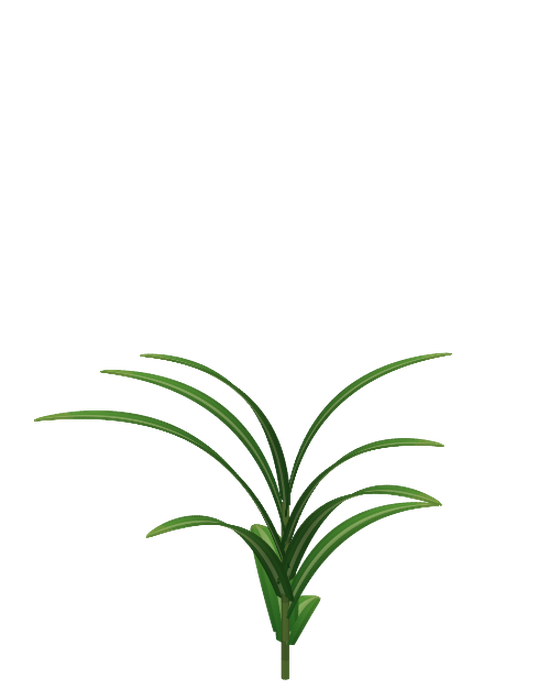
\includegraphics[width=0.7381in, height=0.9327in]{Figures/fig_dataset_stats/sorghum_0.png}};
\node[anchor=south west, inner sep=0] at (1.1481,3.5452) {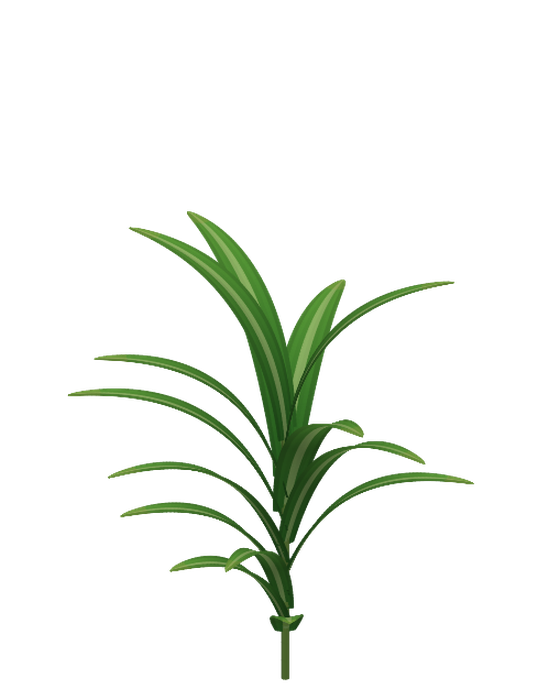
\includegraphics[width=0.7381in, height=0.9327in]{Figures/fig_dataset_stats/sorghum_1.png}};
\node[anchor=south west, inner sep=0] at (1.9763,3.5452) {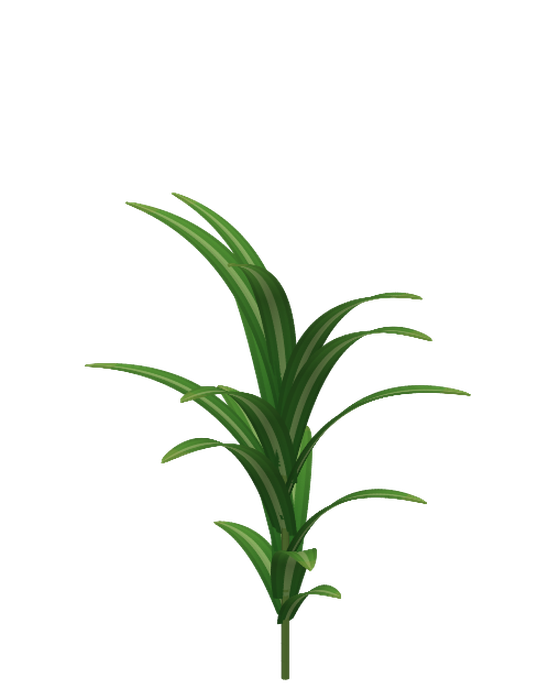
\includegraphics[width=0.7381in, height=0.9327in]{Figures/fig_dataset_stats/sorghum_2.png}};
\node[anchor=south west, inner sep=0] at (2.8044,3.5452) {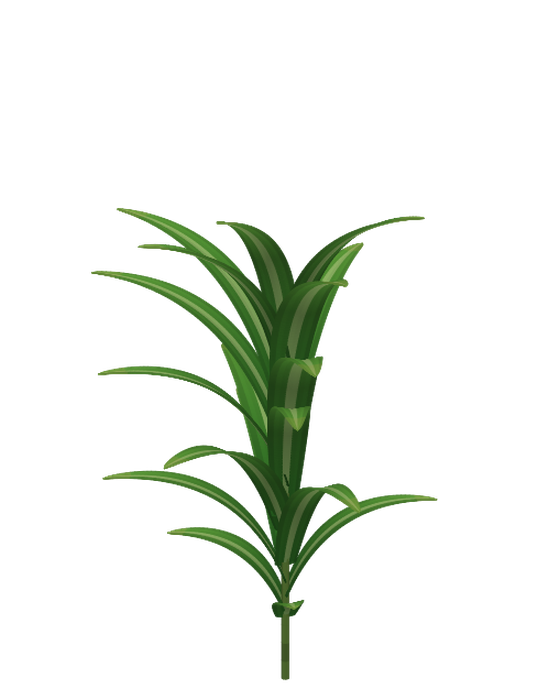
\includegraphics[width=0.7381in, height=0.9327in]{Figures/fig_dataset_stats/sorghum_3.png}};
\node[anchor=south west, inner sep=0] at (3.6325,3.5452) {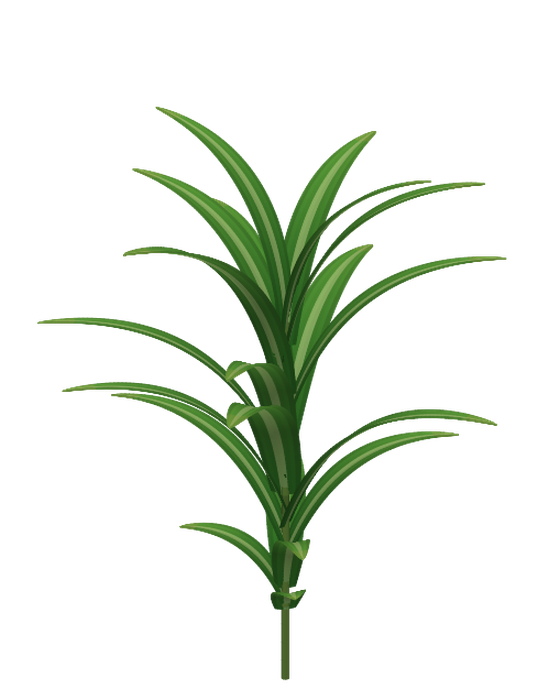
\includegraphics[width=0.7381in, height=0.9327in]{Figures/fig_dataset_stats/sorghum_4.png}};
\node[anchor=south west, inner sep=0] at (4.4606,3.5452) {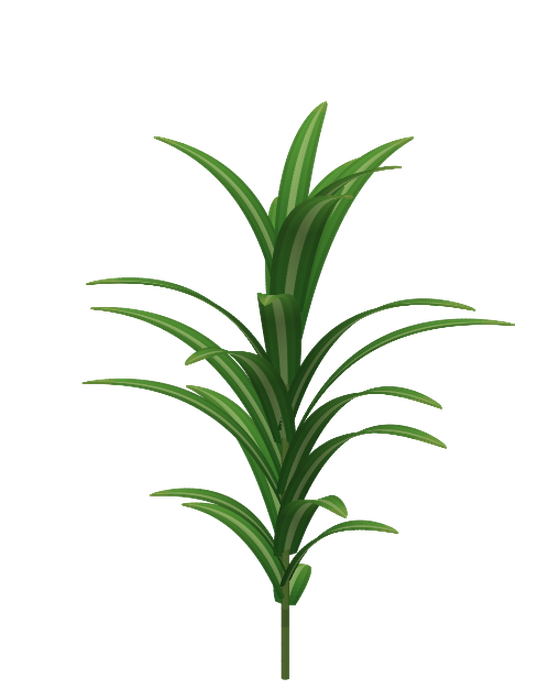
\includegraphics[width=0.7381in, height=0.9327in]{Figures/fig_dataset_stats/sorghum_5.png}};
\node[anchor=south west, inner sep=0] at (5.2888,3.5452) {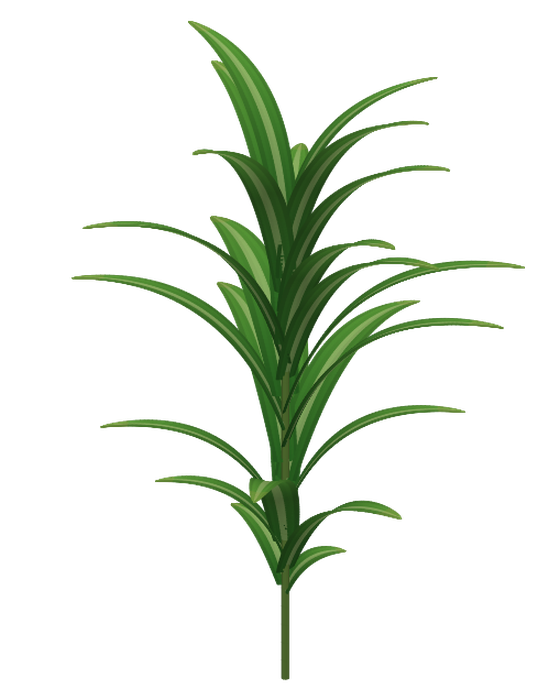
\includegraphics[width=0.7381in, height=0.9327in]{Figures/fig_dataset_stats/sorghum_6.png}};
\node[anchor=south west, inner sep=0] at (6.1169,3.5452) {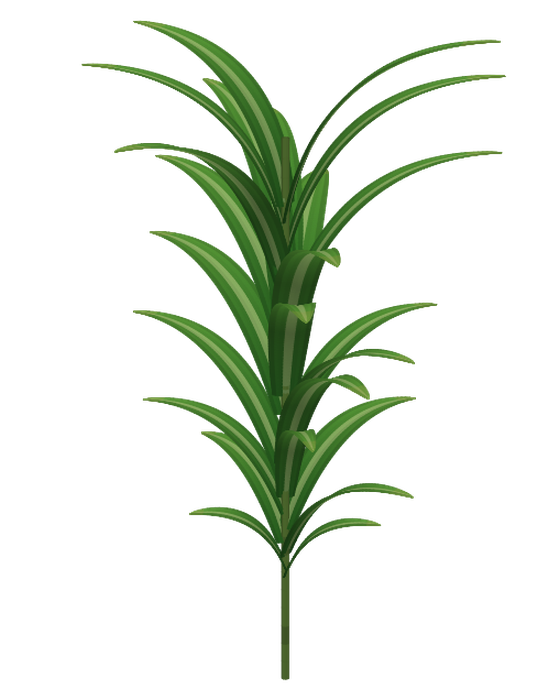
\includegraphics[width=0.7381in, height=0.9327in]{Figures/fig_dataset_stats/sorghum_7.png}};
\node[anchor=south west, inner sep=0] at (0.3200,2.2925) {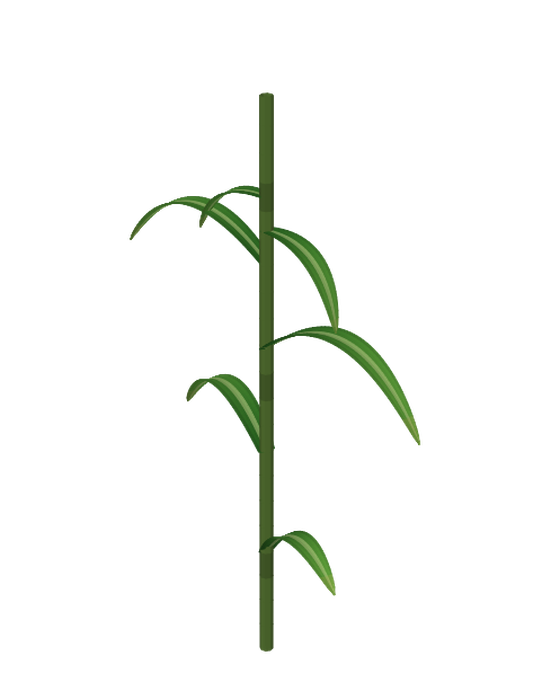
\includegraphics[width=0.7381in, height=0.9327in]{Figures/fig_dataset_stats/maize_0.png}};
\node[anchor=south west, inner sep=0] at (1.1481,2.2925) {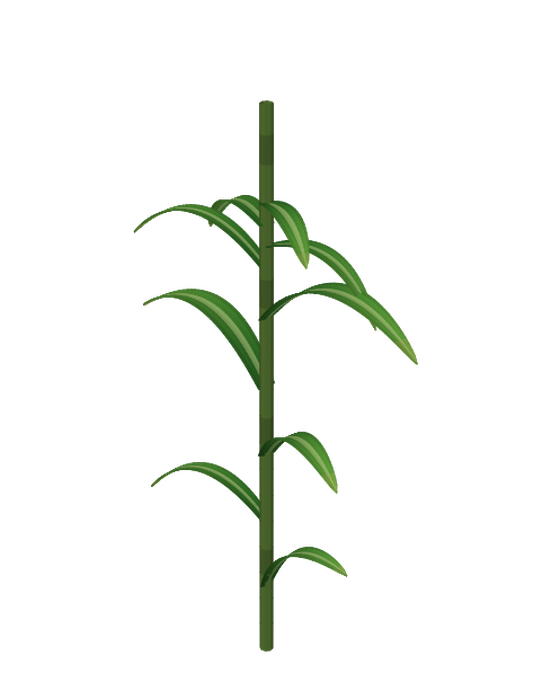
\includegraphics[width=0.7381in, height=0.9327in]{Figures/fig_dataset_stats/maize_1.png}};
\node[anchor=south west, inner sep=0] at (1.9763,2.2925) {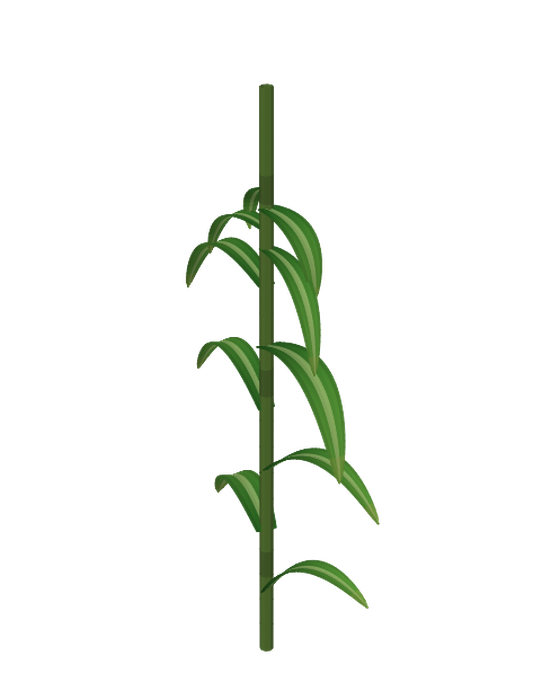
\includegraphics[width=0.7381in, height=0.9327in]{Figures/fig_dataset_stats/maize_2.png}};
\node[anchor=south west, inner sep=0] at (2.8044,2.2925) {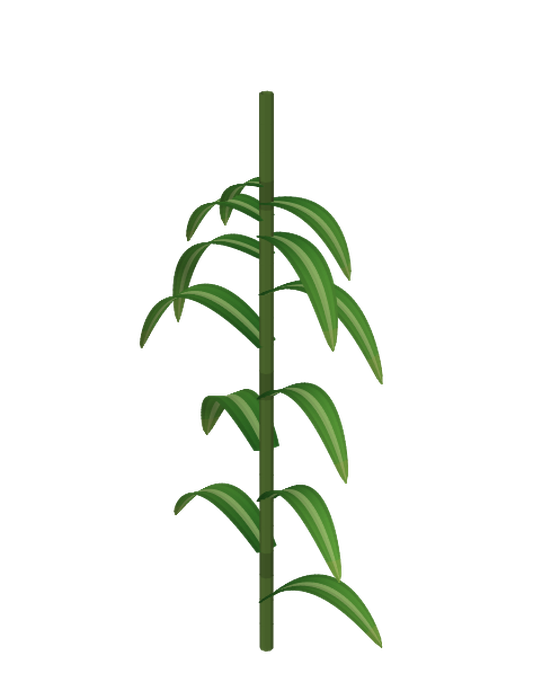
\includegraphics[width=0.7381in, height=0.9327in]{Figures/fig_dataset_stats/maize_3.png}};
\node[anchor=south west, inner sep=0] at (3.6325,2.2925) {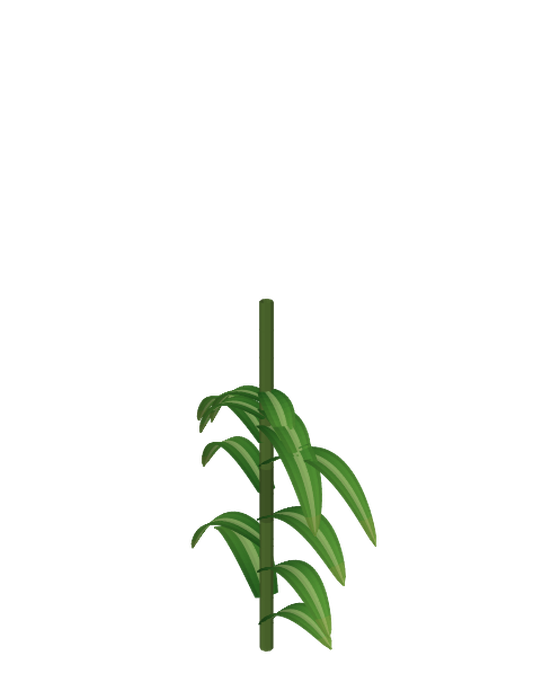
\includegraphics[width=0.7381in, height=0.9327in]{Figures/fig_dataset_stats/maize_4.png}};
\node[anchor=south west, inner sep=0] at (4.4606,2.2925) {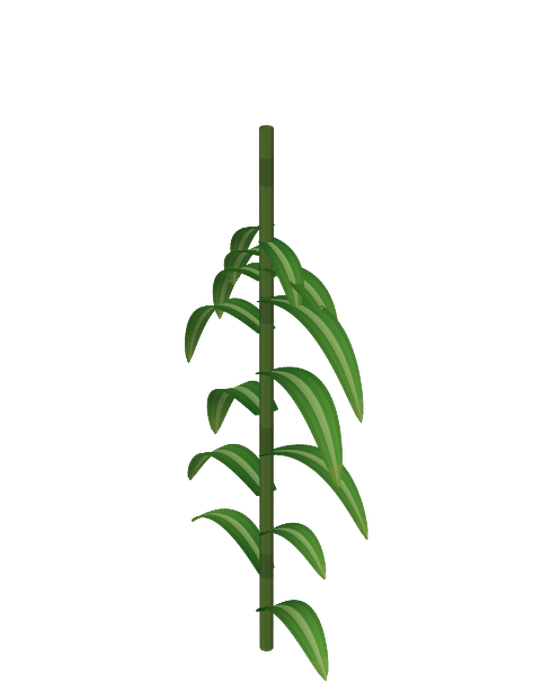
\includegraphics[width=0.7381in, height=0.9327in]{Figures/fig_dataset_stats/maize_5.png}};
\node[anchor=south west, inner sep=0] at (5.2888,2.2925) {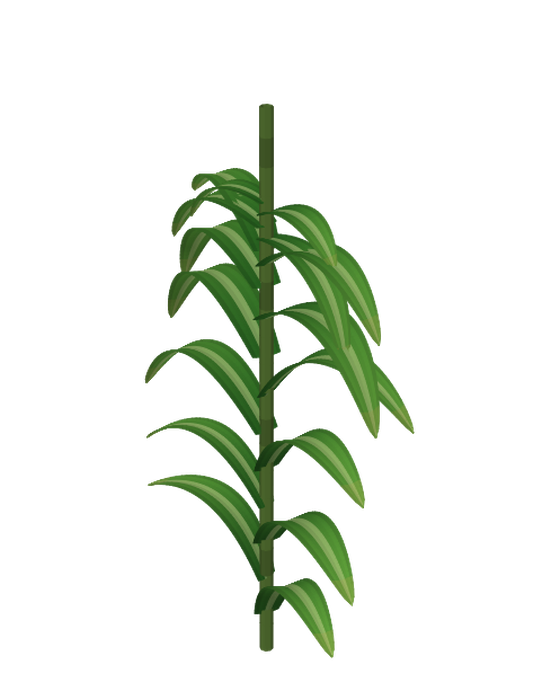
\includegraphics[width=0.7381in, height=0.9327in]{Figures/fig_dataset_stats/maize_6.png}};
\node[anchor=south west, inner sep=0] at (6.1169,2.2925) {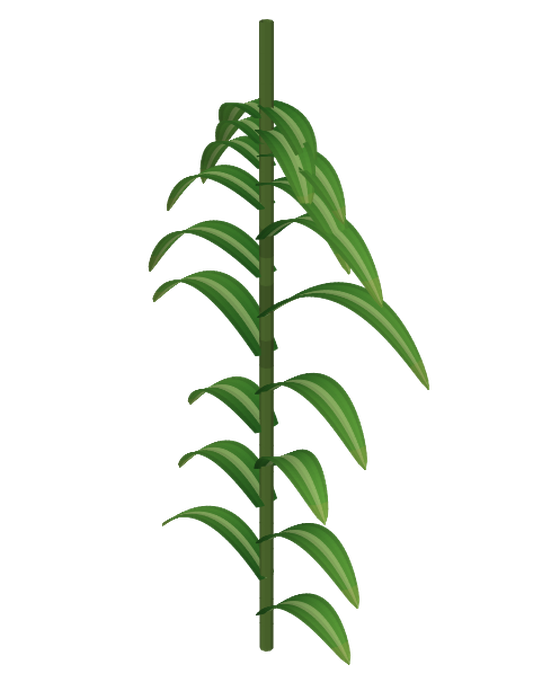
\includegraphics[width=0.7381in, height=0.9327in]{Figures/fig_dataset_stats/maize_7.png}};
\node[anchor=south west, inner sep=0] at (0.0000,0.0200) {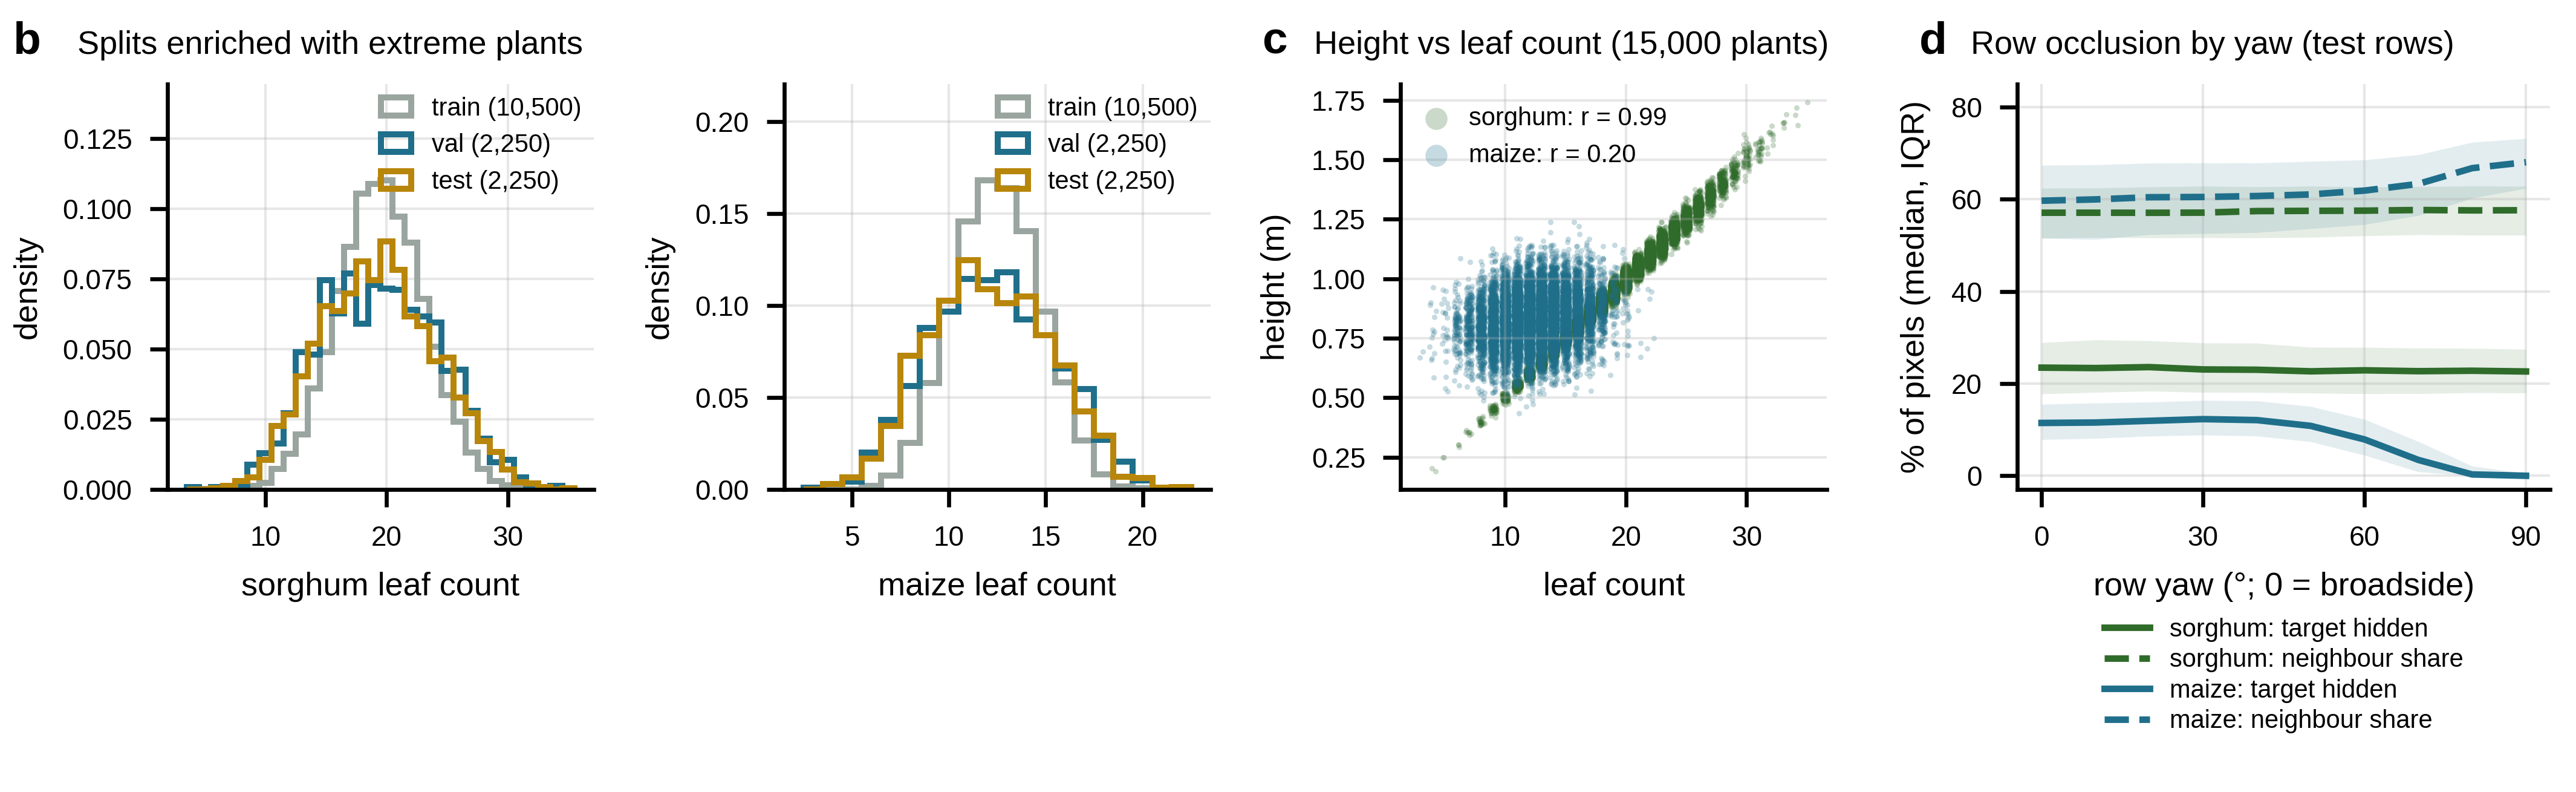
\includegraphics[width=6.8750in, height=2.1125in]{Figures/fig_dataset_stats/panels_b_d.png}};
\node[anchor=north west, inner sep=0, outer sep=0, align=left, text=c1D221C, font={\fontsize{9.00}{11.25}\selectfont\sffamily\bfseries}] at (0.0000,4.8578) {a};
\node[anchor=north west, inner sep=0, outer sep=0, align=left, text=c1D221C, font={\fontsize{6.40}{8.00}\selectfont\sffamily}] at (0.1600,4.8428) {The morphological range: eight val plants per species along the leaf-count range (sorghum 4--35 leaves, maize 3--22), true procedural models};
\node[anchor=south, inner sep=0, outer sep=0, align=center, text=c1D221C, font={\fontsize{6.00}{7.50}\selectfont\sffamily}] at (0.6891,4.5278) {10 leaves, 0.50 m};
\node[anchor=south, inner sep=0, outer sep=0, align=center, text=c1D221C, font={\fontsize{6.00}{7.50}\selectfont\sffamily}] at (1.5172,4.5278) {14 leaves, 0.68 m};
\node[anchor=south, inner sep=0, outer sep=0, align=center, text=c1D221C, font={\fontsize{6.00}{7.50}\selectfont\sffamily}] at (2.3453,4.5278) {16 leaves, 0.81 m};
\node[anchor=south, inner sep=0, outer sep=0, align=center, text=c1D221C, font={\fontsize{6.00}{7.50}\selectfont\sffamily}] at (3.1734,4.5278) {18 leaves, 0.88 m};
\node[anchor=south, inner sep=0, outer sep=0, align=center, text=c1D221C, font={\fontsize{6.00}{7.50}\selectfont\sffamily}] at (4.0016,4.5278) {20 leaves, 0.99 m};
\node[anchor=south, inner sep=0, outer sep=0, align=center, text=c1D221C, font={\fontsize{6.00}{7.50}\selectfont\sffamily}] at (4.8297,4.5278) {22 leaves, 1.06 m};
\node[anchor=south, inner sep=0, outer sep=0, align=center, text=c1D221C, font={\fontsize{6.00}{7.50}\selectfont\sffamily}] at (5.6578,4.5278) {25 leaves, 1.25 m};
\node[anchor=south, inner sep=0, outer sep=0, align=center, text=c1D221C, font={\fontsize{6.00}{7.50}\selectfont\sffamily}] at (6.4859,4.5278) {29 leaves, 1.48 m};
\node[anchor=center, inner sep=0, outer sep=0, align=center, text=c1D221C, font={\fontsize{6.60}{8.25}\selectfont\sffamily}, rotate=90] at (0.1000,4.0115) {sorghum};
\node[anchor=south, inner sep=0, outer sep=0, align=center, text=c1D221C, font={\fontsize{6.00}{7.50}\selectfont\sffamily}] at (0.6891,3.2752) {6 leaves, 0.88 m};
\node[anchor=south, inner sep=0, outer sep=0, align=center, text=c1D221C, font={\fontsize{6.00}{7.50}\selectfont\sffamily}] at (1.5172,3.2752) {9 leaves, 0.87 m};
\node[anchor=south, inner sep=0, outer sep=0, align=center, text=c1D221C, font={\fontsize{6.00}{7.50}\selectfont\sffamily}] at (2.3453,3.2752) {10 leaves, 0.90 m};
\node[anchor=south, inner sep=0, outer sep=0, align=center, text=c1D221C, font={\fontsize{6.00}{7.50}\selectfont\sffamily}] at (3.1734,3.2752) {12 leaves, 0.90 m};
\node[anchor=south, inner sep=0, outer sep=0, align=center, text=c1D221C, font={\fontsize{6.00}{7.50}\selectfont\sffamily}] at (4.0016,3.2752) {13 leaves, 0.52 m};
\node[anchor=south, inner sep=0, outer sep=0, align=center, text=c1D221C, font={\fontsize{6.00}{7.50}\selectfont\sffamily}] at (4.8297,3.2752) {14 leaves, 0.83 m};
\node[anchor=south, inner sep=0, outer sep=0, align=center, text=c1D221C, font={\fontsize{6.00}{7.50}\selectfont\sffamily}] at (5.6578,3.2752) {16 leaves, 0.87 m};
\node[anchor=south, inner sep=0, outer sep=0, align=center, text=c1D221C, font={\fontsize{6.00}{7.50}\selectfont\sffamily}] at (6.4859,3.2752) {19 leaves, 1.05 m};
\node[anchor=center, inner sep=0, outer sep=0, align=center, text=c1D221C, font={\fontsize{6.60}{8.25}\selectfont\sffamily}, rotate=90] at (0.1000,2.7589) {maize};
\end{tikzpicture}%
}%
